\documentclass[11pt]{beamer}

\usetheme{Darmstadt}

\usepackage{times}
\usefonttheme{structurebold}

\usepackage[english]{babel}
\usepackage{pgf,pgfarrows,pgfnodes,pgfautomata,pgfheaps}
\usepackage{amsmath,amssymb}
\usepackage[latin1]{inputenc}
\usepackage{multicol}

%
%  This version the file slabbrev.tex is designed to work with
%  the beamer package
%

\newcommand{\ns}{
  \end{slide}
  \begin{slide}
  \sffamily
}
\newcommand{\bs}{
  \begin{slide}
  \sffamily
}
\newcommand{\es}{
  \end{slide}
}

\newcommand{\bi}{
  \begin{itemize}
}

\newcommand{\ei}{
  \end{itemize}
}

%
%  Inner product macro
%
\newcommand{\IP}[2]{ \langle #1 , #2 \rangle }
%
\newcommand{\twobytwo}[4]{\left ( \begin{array}{cc}#1&#2\\#3&#4 \end{array}
\right ) }
\newcommand{\twobyone}[2]{\left ( \begin{array}{c}#1 \\ #2 \end{array}
\right ) }
\newcommand{\twobytwob}[4]{\left [ \! \begin{array}{cc}#1&#2\\#3&#4 \end{array}
\! \right ] }
\newcommand{\twobyoneb}[2]{\left [\! \begin{array}{c}#1 \\ #2 \end{array}
\! \right ] }
\renewcommand{\ne}{\! \not \, = }
\newcommand{\be}[1]{\begin{equation}\label{#1}}
\newcommand{\ee}{\end{equation}}
\newcommand{\cJ}{{\cal J}}
\newcommand{\cK}{{\cal K}}
\newcommand{\cM}{{\cal M}}
\newcommand{\cS}{{\cal S}}
\newcommand{\cT}{{\cal T}}
\newcommand{\cV}{{\cal V}}
\newcommand{\cZ}{{\cal Z}}
\newcommand{\muh}{\hat{\mu}}
\newcommand{\Gamh}{\hat{\Gamma}}
\newcommand{\gamh}{\hat{\gamma}}
\newcommand{\gamt}{\tilde{\gamma}}
\newcommand{\xit}{\tilde{\xi}}
\newcommand{\ut}{\tilde{u}}
\newcommand{\vt}{\tilde{v}}
\newcommand{\lamh}{\hat{\lambda}}
\newcommand{\gamb}{\mbox{\boldmath$\gamma$}}
\newcommand{\Gamb}{\mbox{\boldmath$\Gamma$}}
\newcommand{\betb}{\mbox{\boldmath$\beta$}}
\newcommand{\bX}{{\bf X}}
\newcommand{\bg}{{\bf g}}

\newcommand{\Ddo}   {\mbox{D}}
\newcommand{\Ldo}   {\mbox{L}}

\newcommand{\ROUPEN}   {\mbox{\tt ROUPEN}}
\newcommand{\PEN}      {\mbox{\tt PEN}}
\newcommand{\PENRSS}   {\mbox{\tt PENRSS}}
\newcommand{\REGSSE}   {\mbox{\tt REGSSE}}
\newcommand{\PCASSE}   {\mbox{\tt PCASSE}}
\newcommand{\PCAPSV}   {\mbox{\tt PCAPSV}}
\newcommand{\LMSSE}    {\mbox{\tt LMSSE}}
\newcommand{\PENSSE}   {\mbox{\tt PENSSE}}
\newcommand{\SMPENSSE} {\mbox{\tt SMPENSSE}}
\newcommand{\RSQ}      {\mbox{\tt RSQ}}
\newcommand{\FRATIO}   {\mbox{\tt FRATIO}}
\newcommand{\SMSSE}    {\mbox{\tt SMSSE}}
\newcommand{\LOCSSE}   {\mbox{\tt SMLOCSSE}}
\newcommand{\Kern}     {\mbox{\tt Kern}}
\newcommand{\Triang}   {\mbox{\tt Triang}}
\newcommand{\cov}      {\mbox{\tt cov}}
\newcommand{\corr}     {\mbox{\tt corr}}
\newcommand{\var}      {\mbox{\tt var}}
\newcommand{\GCV}      {\mbox{\tt GCV}}
\newcommand{\CV}       {\mbox{\tt CV}}
\newcommand{\DF}       {\mbox{\tt DF}}
\newcommand{\GFR}      {{\tt GFR}}
\newcommand{\GOP}      {{\tt GOP}}
\newcommand{\KUC}      {{\tt KUC}}
\newcommand{\LMISE}    {\mbox{\tt LMISE}}
\newcommand{\sign}     {\mbox{\tt sign}}
\newcommand{\MINEIG}   {\mbox{\tt MINEIG}}
\newcommand{\Height}   {\mbox{\tt Height}}
\newcommand{\Acceleration}   {\mbox{\tt Acceleration}}
\newcommand{\Temp}     {\mbox{\tt Temp}}
\newcommand{\Prec}     {\mbox{\tt Prec}}
\newcommand{\Precmn}   {\mbox{\tt Precmn}}
\newcommand{\Precstar} {\mbox{{\tt Prec}^{*}}}
\newcommand{\LPrec}    {\mbox{\tt LPrec}}
\newcommand{\Hi}       {\mbox{\footnotesize \tt H}}
\newcommand{\Kn}       {\mbox{\footnotesize \tt K}}
\newcommand{\Hipsmall}  {\mbox{\footnotesize \tt Hip}}
\newcommand{\Kneesmall} {\mbox{\footnotesize \tt Knee}}
\newcommand{\Hip}      {\mbox{\tt Hip}}
\newcommand{\Knee}     {\mbox{\tt Knee}}
\newcommand{\Hipmn}    {\mbox{\tt Hipmn}}
\newcommand{\Kneemn}   {\mbox{\tt Kneemn}}
\newcommand{\Angles}   {\mbox{\tt Angles}}
\newcommand{\ScriptX}  {\mbox{\tt ScriptX}}
\newcommand{\ScriptY}  {\mbox{\tt ScriptY}}
\newcommand{\GDP}      {\mbox{\tt GDP}}
\newcommand{\Bias}     {\mbox{\tt Bias}}
\newcommand{\IMSE}     {\mbox{\tt IMSE}}
\newcommand{\RMSE}     {\mbox{\tt RMSE}}
\newcommand{\Var}      {\mbox{\tt Var}}
\newcommand{\Stt}      {\mbox{\tt S}}
\newcommand{\Ctt}      {\mbox{\tt C}}
\newcommand{\SSE}      {\mbox{\tt SSE}}
\newcommand{\SSY}      {\mbox{\tt SSY}}
\newcommand{\SAD}      {\mbox{\tt SAD}}
\newcommand{\MSE}   {\mbox{\tt MSE}}
\newcommand{\PSSE}  {\mbox{\tt PSSE}}
\newcommand{\MSR}   {\mbox{\tt MSR}}
\newcommand{\tPDA}  {\mbox{\tiny PDA}}
\newcommand{\tPCA}  {\mbox{\tiny PCA}}
\newcommand{\Force} {\mbox{\tt Force}}
\newcommand{\ForceX}    {\mbox{\tt ForceX}}
\newcommand{\ForceY}    {\mbox{\tt ForceY}}
\newcommand{\Contrast}  {\mbox{\tt Contrast}}

\newcommand{\rhat}     {\hat{r}}
\newcommand{\uhat}     {\hat{u}}
\newcommand{\vhat}     {\hat{v}}
\newcommand{\xhat}     {\hat{x}}
\newcommand{\yhat}     {\hat{y}}
\newcommand{\Fhat}     {\hat{F}}
\newcommand{\Mhat}     {\hat{M}}
\newcommand{\alphahat} {\hat{\alpha}}
\newcommand{\betahat}  {\hat{\beta}}

\newcommand{\xtilde}   {\tilde{x}}
\newcommand{\etilde}   {\tilde{e}}
\newcommand{\ktilde}   {\tilde{k}}

\newcommand{\lcal}     {\ell}
\newcommand{\Bcal}     {\mbox{$\cal B$}}
\newcommand{\Fcal}     {\mbox{$\cal F$}}
\newcommand{\Gcal}     {\mbox{$\cal G$}}
\newcommand{\Hcal}     {\mbox{$\cal H$}}
\newcommand{\Lcal}     {\mbox{$\cal L$}}
\newcommand{\Pcal}     {\mbox{$\cal P$}}
\newcommand{\Rcal}     {\mbox{$\cal R$}}
\newcommand{\Tcal}     {\mbox{$\cal T$}}
\newcommand{\Ucal}     {\mbox{$\cal U$}}
\newcommand{\Ycal}     {\mbox{$\cal Y$}}

\newcommand{\TcalX}     {{{\cal T}_{\!X}}}
\newcommand{\TcalY}     {{{\cal T}_{\!Y}}}


\newcommand{\spann}    {\mbox{span}}
\newcommand{\diag}     {\mbox{diag}}
\newcommand{\Exp}      {\mbox{E}}

\newcommand{\abold}    {\mbox{\bf a}}
\newcommand{\bbold}    {\mbox{\bf b}}
\newcommand{\cbold}    {\mbox{\bf c}}
\newcommand{\dbold}    {\mbox{\bf d}}
\newcommand{\ebold}    {\mbox{\bf e}}
\newcommand{\fbold}    {\mbox{\bf f}}
\newcommand{\gbold}    {\mbox{\bf g}}
\newcommand{\hbold}    {\mbox{\bf h}}
\newcommand{\kbold}    {\mbox{\bf k}}
\newcommand{\rbold}    {\mbox{\bf r}}
\newcommand{\sbold}    {\mbox{\bf s}}
\newcommand{\tbold}    {\mbox{\bf t}}
\newcommand{\ubold}    {\mbox{\bf u}}
\newcommand{\vbold}    {\mbox{\bf v}}
\newcommand{\wbold}    {\mbox{\bf w}}
\newcommand{\xbold}    {\mbox{\bf x}}
\newcommand{\ybold}    {\mbox{\bf y}}
\newcommand{\zbold}    {\mbox{\bf z}}
\newcommand{\Abold}    {\mbox{\bf A}}
\newcommand{\Bbold}    {\mbox{\bf B}}
\newcommand{\Cbold}    {\mbox{\bf C}}
\newcommand{\Dbold}    {\mbox{\bf D}}
\newcommand{\Ebold}    {\mbox{\bf E}}
\newcommand{\Fbold}    {\mbox{\bf F}}
\newcommand{\Gbold}    {\mbox{\bf G}}
\newcommand{\Hbold}    {\mbox{\bf H}}
\newcommand{\Ibold}    {\mbox{\bf I}}
\newcommand{\Jbold}    {\mbox{\bf J}}
\newcommand{\Kbold}    {\mbox{\bf K}}
\newcommand{\Lbold}    {\mbox{\bf L}}
\newcommand{\Mbold}    {\mbox{\bf M}}
\newcommand{\Nbold}    {\mbox{\bf N}}
\newcommand{\Pbold}    {\mbox{\bf P}}
\newcommand{\Qbold}    {\mbox{\bf Q}}
\newcommand{\Rbold}    {\mbox{\bf R}}
\newcommand{\Sbold}    {\mbox{\bf S}}
\newcommand{\Tbold}    {\mbox{\bf T}}
\newcommand{\Ubold}    {\mbox{\bf U}}
\newcommand{\Vbold}    {\mbox{\bf V}}
\newcommand{\Wbold}    {\mbox{\bf W}}
\newcommand{\Xbold}    {\mbox{\bf X}}
\newcommand{\Ybold}    {\mbox{\bf Y}}
\newcommand{\Zbold}    {\mbox{\bf Z}}


\newcommand{\onebold}   {\mbox{\bf 1}}
\newcommand{\zerobold}  {\mbox{\bf 0}}

\newcommand{\xhatbold} {\hat{\mbox{\bf x}}}
\newcommand{\yhatbold} {\hat{\mbox{\bf y}}}
\newcommand{\Ahatbold} {\hat{\mbox{\bf A}}}
\newcommand{\Bhatbold} {\hat{\mbox{\bf B}}}
\newcommand{\Qhatbold} {\hat{\mbox{\bf Q}}}
\newcommand{\Rhatbold} {\hat{\mbox{\bf R}}}
\newcommand{\Yhatbold} {\hat{\mbox{\bf Y}}}

\newcommand{\cboldhat}    {\hat{\mbox{\bf c}}}

\newcommand{\alphabold}   {\mbox{\boldmath${\alpha}$}}
\newcommand{\betabold}    {\mbox{\boldmath${\beta}$}}
\newcommand{\deltabold}   {\mbox{\boldmath${\delta}$}}
\newcommand{\Deltabold}   {\mbox{\boldmath${\Delta}$}}
\newcommand{\epsilonbold} {\mbox{\boldmath${\epsilon}$}}
\newcommand{\gammabold}   {\mbox{\boldmath${\gamma}$}}
\newcommand{\lambdabold}  {\mbox{\boldmath${\lambda}$}}
\newcommand{\Lambdabold}  {\mbox{\boldmath${\Lambda}$}}
\newcommand{\mubold}      {\mbox{\boldmath${\mu}$}}
\newcommand{\thetabold}   {\mbox{\boldmath${\theta}$}}
\newcommand{\phibold}     {\mbox{\boldmath${\phi}$}}
\newcommand{\Phibold}     {\mbox{\boldmath${\Phi}$}}
\newcommand{\psibold}     {\mbox{\boldmath${\psi}$}}
\newcommand{\Psibold}     {\mbox{\boldmath${\Psi}$}}
\newcommand{\Sigb}        {\mbox{\boldmath${\Sigma}$}}
\newcommand{\xibold}      {\mbox{\boldmath${\xi}$}}

\newcommand{\thetaboldhat} {\hat{\mbox{\boldmath${\theta}$}}}

\newcommand{\xbar}     {\bar{x}}
\newcommand{\ybar}     {\bar{y}}
\newcommand{\Pbar}     {\bar{P}}

\newcommand{\gtilde}       {\tilde{g}}
\newcommand{\ntilde}       {\tilde{n}}
\newcommand{\alphatilde}   {\tilde{\alpha}}
\newcommand{\betatilde}    {\tilde{\beta}}

\newcommand{\estar}    {e^{*}}
\newcommand{\fstar}    {f^{*}}
\newcommand{\ustar}    {u^{*}}
\newcommand{\vstar}    {v^{*}}
\newcommand{\xstar}    {x^{*}}
\newcommand{\ystar}    {y^{*}}
\newcommand{\Astar}    {A^{*}}
\newcommand{\Bstar}    {B^{*}}
\newcommand{\Estar}    {E^{*}}
\newcommand{\Fstar}    {F^{*}}
\newcommand{\Lstar}    {L^{*}}
\newcommand{\Pstar}    {P^{*}}
\newcommand{\Ustar}    {U^{*}}
\newcommand{\Vstar}    {V^{*}}
\newcommand{\Xstar}    {X^{*}}

\newcommand{\eperp}     {e^{\bot}}
\newcommand{\xboldstar}{ {\mbox{\bf x}}^{*}}
\newcommand{\yboldstar}{ {\mbox{\bf y}}^{*}}
\newcommand{\ystarhat}{ \hat{y}^{*}}
\newcommand{\yboldstarhat}{ \hat{\mbox{\bf y}}^{*}}

\newcommand{\betastar} {\beta^{*}}
\newcommand{\etastar}  {\eta^{*}}

\newcommand{\Pbarstar} {\bar{P}^{*}}

\newcommand{\Aplus}    {A^{+}}

\newcommand{\Amins}    {A^{-}}
\newcommand{\Xmins}    {X^{-}}
\newcommand{\Zmins}    {Z^{-}}

\newcommand{\Zinv}     {Z^{-1}}
\newcommand{\Zginv}    {Z^{-}}


\newcommand{\Zboldinv} {\mbox{\bf Z}^{-1}}

\newcommand{\Qboldginv}{\mbox{\bf Q}^{-}}
\newcommand{\Rboldginv}{\mbox{\bf R}^{-}}
\newcommand{\Zboldginv}{\mbox{\bf Z}^{-}}

\newcommand{\rank}     {\mbox{rank}}
\newcommand{\trace}    {\mbox{trace}}

\newcommand{\smint}{\! \int \!}
\newcommand{\Gambt}{\tilde{\mbox{\boldmath${\Gamma}$}}}

\newcommand{\cvu}{a}
\newcommand{\cvv}{b}
\newcommand{\cfu}{\xi}
\newcommand{\cfv}{\eta}
\newcommand{\Vboldt}{\tilde{\Vbold}}
\newcommand{\funcov}{v}
\newcommand{\funcovh}{\hat{v}}
\newcommand{\Funcov}{V}
\newcommand{\Funcovh}{\hat{V}}
\newcommand{\cancov}{{\mbox{\tt ccorsq}}^{pop}}
\newcommand{\cancovh}{\mbox{\tt ccorsq}}

\newcommand{\Splus}{S-PLUS}
\newcommand{\df}{\mbox{\tt df}}
\newcommand{\etal}{et al.\ }

\setbeamercovered{dynamic}

\newcommand{\Lang}[1]{\operatorname{\text{\textsc{#1}}}}

\newcommand{\Class}[1]{\operatorname{\mathchoice
  {\text{\sf \small #1}}
  {\text{\sf \small #1}}
  {\text{\sf #1}}
  {\text{\sf #1}}}}

\newcommand{\NumSAT}      {\text{\small\#SAT}}
\newcommand{\NumA}        {\#_{\!A}}

\newcommand{\barA}        {\,\bar{\!A}}

\newcommand{\Nat}{\mathbb{N}}
\newcommand{\Set}[1]{\{#1\}}

\pgfdeclaremask{tu}{beamer-tu-logo-mask} \pgfdeclaremask{computer}{beamer-computer-mask}
\pgfdeclareimage[interpolate=true,mask=computer,height=2cm]{computerimage}{beamer-computer}
\pgfdeclareimage[interpolate=true,mask=computer,height=2cm]{computerworkingimage}{beamer-computerred}
\pgfdeclareimage[mask=tu,height=.5cm]{logo}{beamer-tu-logo}

%\logo{\pgfuseimage{logo}}

\colorlet{redshaded}{red!25!bg} \colorlet{shaded}{black!25!bg} \colorlet{shadedshaded}{black!10!bg}
\colorlet{blackshaded}{black!40!bg}

\colorlet{darkred}{red!80!black} \colorlet{darkblue}{blue!80!black}
\colorlet{darkgreen}{green!80!black}

\def\radius{0.96cm}
\def\innerradius{0.85cm}

\def\softness{0.4}
\definecolor{softred}{rgb}{1,\softness,\softness}
\definecolor{softgreen}{rgb}{\softness,1,\softness}
\definecolor{softblue}{rgb}{\softness,\softness,1}

\definecolor{softrg}{rgb}{1,1,\softness}
\definecolor{softrb}{rgb}{1,\softness,1}
\definecolor{softgb}{rgb}{\softness,1,1}

\newcommand{\Bandshaded}[2]{
  \color{shadedshaded}
  \pgfmoveto{\pgfxy(-0.5,0)}
  \pgflineto{\pgfxy(-0.6,0.1)}
  \pgflineto{\pgfxy(-0.4,0.2)}
  \pgflineto{\pgfxy(-0.6,0.3)}
  \pgflineto{\pgfxy(-0.4,0.4)}
  \pgflineto{\pgfxy(-0.5,0.5)}
  \pgflineto{\pgfxy(4,0.5)}
  \pgflineto{\pgfxy(4.1,0.4)}
  \pgflineto{\pgfxy(3.9,0.3)}
  \pgflineto{\pgfxy(4.1,0.2)}
  \pgflineto{\pgfxy(3.9,0.1)}
  \pgflineto{\pgfxy(4,0)}
  \pgfclosepath
  \pgffill

  \color{black}
  \pgfputat{\pgfxy(0,0.7)}{\pgfbox[left,base]{#1}}
  \pgfputat{\pgfxy(0,-0.1)}{\pgfbox[left,top]{#2}}
}

\newcommand{\Band}[2]{
  \color{shaded}
  \pgfmoveto{\pgfxy(-0.5,0)}
  \pgflineto{\pgfxy(-0.6,0.1)}
  \pgflineto{\pgfxy(-0.4,0.2)}
  \pgflineto{\pgfxy(-0.6,0.3)}
  \pgflineto{\pgfxy(-0.4,0.4)}
  \pgflineto{\pgfxy(-0.5,0.5)}
  \pgflineto{\pgfxy(4,0.5)}
  \pgflineto{\pgfxy(4.1,0.4)}
  \pgflineto{\pgfxy(3.9,0.3)}
  \pgflineto{\pgfxy(4.1,0.2)}
  \pgflineto{\pgfxy(3.9,0.1)}
  \pgflineto{\pgfxy(4,0)}
  \pgfclosepath
  \pgffill

  \color{black}
  \pgfputat{\pgfxy(0,0.7)}{\pgfbox[left,base]{#1}}
  \pgfputat{\pgfxy(0,-0.1)}{\pgfbox[left,top]{#2}}
}

\newcommand{\BaenderNormal}
{%
  \pgfsetlinewidth{0.4pt}
  \color{black}
  \pgfputat{\pgfxy(0,5)}{\Band{input tapes}{}}
  \pgfputat{\pgfxy(0.35,4.6)}{\pgfbox[center,base]{$\vdots$}}
  \pgfputat{\pgfxy(0,4)}{\Band{}{}}

  \pgfxyline(0,5)(0,5.5)
  \pgfxyline(1.2,5)(1.2,5.5)
  \pgfputat{\pgfxy(0.25,5.25)}{\pgfbox[left,center]{$w_1$}}

  \pgfxyline(0,4)(0,4.5)
  \pgfxyline(1.8,4)(1.8,4.5)
  \pgfputat{\pgfxy(0.25,4.25)}{\pgfbox[left,center]{$w_n$}}
  \ignorespaces}

\newcommand{\BaenderZweiNormal}
{%
  \pgfsetlinewidth{0.4pt}
  \color{black}
  \pgfputat{\pgfxy(0,5)}{\Band{Zwei Eingabebänder}{}}
  \pgfputat{\pgfxy(0,4.25)}{\Band{}{}}

  \pgfxyline(0,5)(0,5.5)
  \pgfxyline(1.2,5)(1.2,5.5)
  \pgfputat{\pgfxy(0.25,5.25)}{\pgfbox[left,center]{$u$}}

  \pgfxyline(0,4.25)(0,4.75)
  \pgfxyline(1.8,4.25)(1.8,4.75)
  \pgfputat{\pgfxy(0.25,4.5)}{\pgfbox[left,center]{$v$}}
  \ignorespaces}

\newcommand{\BaenderHell}
{%
  \pgfsetlinewidth{0.4pt}
  \color{black}
  \pgfputat{\pgfxy(0,5)}{\Bandshaded{input tapes}{}}
  \color{shaded}
  \pgfputat{\pgfxy(0.35,4.6)}{\pgfbox[center,base]{$\vdots$}}
  \pgfputat{\pgfxy(0,4)}{\Bandshaded{}{}}

  \color{blackshaded}
  \pgfxyline(0,5)(0,5.5)
  \pgfxyline(1.2,5)(1.2,5.5)
  \pgfputat{\pgfxy(0.25,5.25)}{\pgfbox[left,center]{$w_1$}}

  \pgfxyline(0,4)(0,4.5)
  \pgfxyline(1.8,4)(1.8,4.5)
  \pgfputat{\pgfxy(0.25,4.25)}{\pgfbox[left,center]{$w_n$}}
  \ignorespaces}

\newcommand{\BaenderZweiHell}
{%
  \pgfsetlinewidth{0.4pt}
  \color{black}
  \pgfputat{\pgfxy(0,5)}{\Bandshaded{Zwei Eingabebänder}{}}%
  \color{blackshaded}
  \pgfputat{\pgfxy(0,4.25)}{\Bandshaded{}{}}
  \pgfputat{\pgfxy(0.25,4.5)}{\pgfbox[left,center]{$v$}}
  \pgfputat{\pgfxy(0.25,5.25)}{\pgfbox[left,center]{$u$}}%

  \pgfxyline(0,5)(0,5.5)
  \pgfxyline(1.2,5)(1.2,5.5)

  \pgfxyline(0,4.25)(0,4.75)
  \pgfxyline(1.8,4.25)(1.8,4.75)
  \ignorespaces}

\newcommand{\Slot}[1]{%
  \begin{pgftranslate}{\pgfpoint{#1}{0pt}}%
    \pgfsetlinewidth{0.6pt}%
    \color{structure}%
    \pgfmoveto{\pgfxy(-0.1,5.5)}%
    \pgfbezier{\pgfxy(-0.1,5.55)}{\pgfxy(-0.05,5.6)}{\pgfxy(0,5.6)}%
    \pgfbezier{\pgfxy(0.05,5.6)}{\pgfxy(0.1,5.55)}{\pgfxy(0.1,5.5)}%
    \pgflineto{\pgfxy(0.1,4.0)}%
    \pgfbezier{\pgfxy(0.1,3.95)}{\pgfxy(0.05,3.9)}{\pgfxy(0,3.9)}%
    \pgfbezier{\pgfxy(-0.05,3.9)}{\pgfxy(-0.1,3.95)}{\pgfxy(-0.1,4.0)}%
    \pgfclosepath%
    \pgfstroke%
  \end{pgftranslate}\ignorespaces}

\newcommand{\SlotZwei}[1]{%
  \begin{pgftranslate}{\pgfpoint{#1}{0pt}}%
    \pgfsetlinewidth{0.6pt}%
    \color{structure}%
    \pgfmoveto{\pgfxy(-0.1,5.5)}%
    \pgfbezier{\pgfxy(-0.1,5.55)}{\pgfxy(-0.05,5.6)}{\pgfxy(0,5.6)}%
    \pgfbezier{\pgfxy(0.05,5.6)}{\pgfxy(0.1,5.55)}{\pgfxy(0.1,5.5)}%
    \pgflineto{\pgfxy(0.1,4.25)}%
    \pgfbezier{\pgfxy(0.1,4.25)}{\pgfxy(0.05,4.15)}{\pgfxy(0,4.15)}%
    \pgfbezier{\pgfxy(-0.05,4.15)}{\pgfxy(-0.1,4.2)}{\pgfxy(-0.1,4.25)}%
    \pgfclosepath%
    \pgfstroke%
  \end{pgftranslate}\ignorespaces}

\newcommand{\ClipSlot}[1]{%
  \pgfrect[clip]{\pgfrelative{\pgfxy(-0.1,0)}{\pgfpoint{#1}{4cm}}}{\pgfxy(0.2,1.5)}\ignorespaces}

\newcommand{\ClipSlotZwei}[1]{%
  \pgfrect[clip]{\pgfrelative{\pgfxy(-0.1,0)}{\pgfpoint{#1}{4.25cm}}}{\pgfxy(0.2,1.25)}\ignorespaces}


\AtBeginSection[]{\frame{\frametitle{Outline}\tableofcontents[current]}}


\title{Multivariate and Functional Principal Components without Eigenanalysis}

\author{Jim Ramsay, McGill University \\
        (Alois Kneip, University of Bonn) \\
      International Society of Nonparametric Statistics \\
      Cadiz, Spain \\
      13 June 2014}
\date{}

\begin{document}

\begin{frame}

\maketitle

\end{frame}

\begin{frame}

\begin{center}
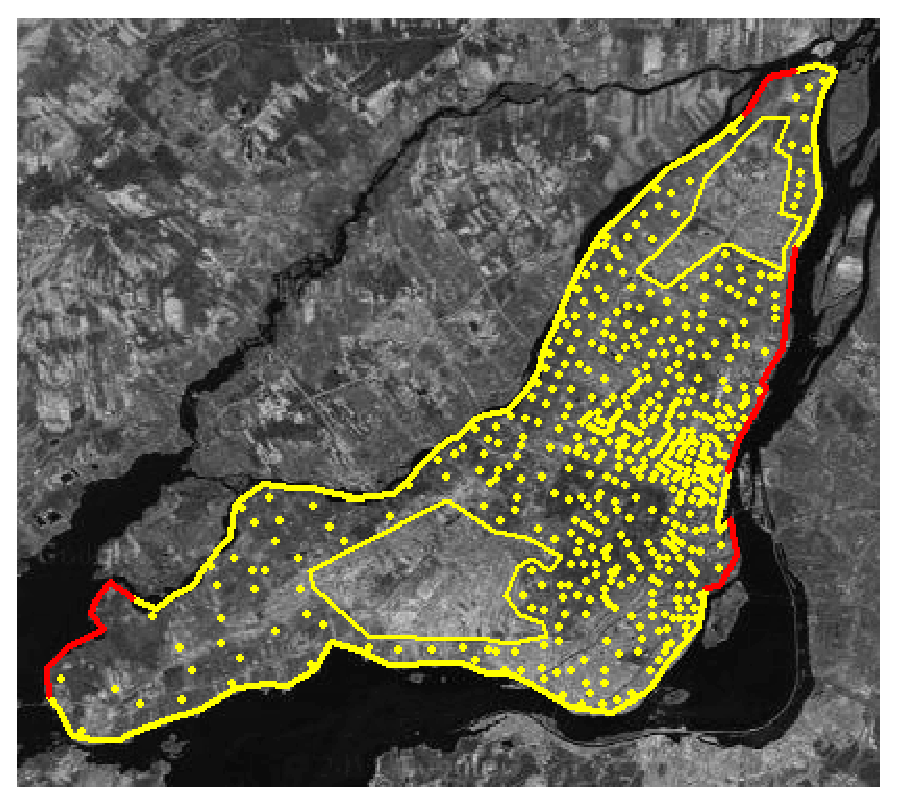
\includegraphics[height=3in, width=4in]{figs/Montreal_data_boundary_small.eps}
\end{center}

\end{frame}

\begin{frame}

Sangalli, L. M., Ramsay, J. O. and Ramsay, T. O. (2013) Spatial spline regression models. \emph{Journal of the Royal Statistical Society, Series B,} {\bf 75}, 681-703.

\end{frame}

\begin{frame}

\begin{center}
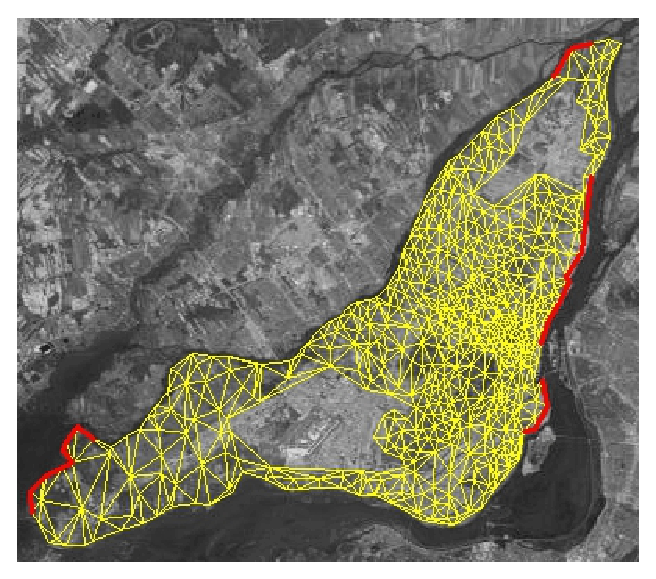
\includegraphics[height=3in, width=4in]{figs/fig_Montreal_triangulation_dirichlet_small.eps}
\end{center}

\end{frame}

\begin{frame}

\begin{center}
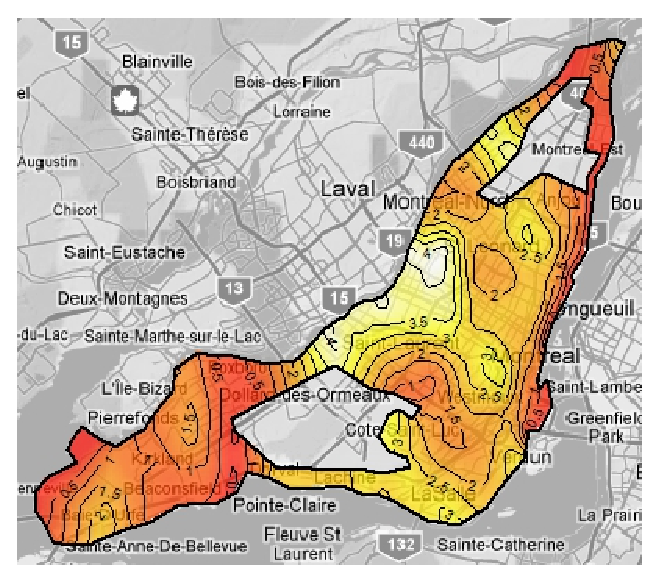
\includegraphics[height=3in, width=4in]{figs/fig_Montreal_results_dirichlet_small_ter.eps}
\end{center}

\end{frame}

%  --------------------------------------------------------------------

\begin{frame}

\frametitle{PCA: The essential idea (Multivariate Case)}

\bi
  \item We have a $N$ by $n$ data matrix $\Xbold$.
  \item We propose the reduced rank $K$ bilinear model
  \[
    \Xbold = \Fbold \Abold
  \]
  \item where $\Abold$ is a $K$ by $n$ matrix of principal component coefficients, with $K << n$
  \item and $\Fbold$ is a $N$ by $K$ matrix of principal component scores
   \item Usually $N >> n$, and the factor scores are interesting, but it's $\Abold$ that tells
  us what the core $K$ components of variation are, to within a full rank linear transformation.
  \item The fundamental goal of PCA is to identify the optimal linear subspace $\cal{R}^K$, called a Grassmann manifold.
\ei

\end{frame}

%  --------------------------------------------------------------------

\begin{frame}

\frametitle{PCA: The essential idea (Functional Case)}

\bi
  \item We have a $N$ curves $x_i(t)$.
  \item We propose the reduced rank $K$ bilinear model
  \[
    \xbold(t) = \Fbold \abold'(t)
  \]
  \item where $\abold$ is a vector $K$ principal component functions, and
  \item and $\Fbold$ is a $N$ by $K$ matrix of principal component scores.
  \item The fundamental goal of PCA is to identify the optimal linear subspace of functions 
  $\abold$.
\ei

\end{frame}

%  --------------------------------------------------------------------

\begin{frame}

\frametitle{Structural parameters}

\bi
  \item Structural parameters are typically of direct interest, for example fixed effect parameters for ME models.
  \item Their number is usually fixed, and typically much smaller than the number of nuisance parameters.
  \item Principal loading matrix $\Abold$ is a structural parameter in multivariate PCA.
\ei

\end{frame}

%  --------------------------------------------------------------------

\begin{frame}

\frametitle{Nuisance parameters}

\bi
  \item Nuisance parameters are required in a model to capture important variation, but are seldom themselves of direct interest.  A well-known example are random effect parameters in a mixed effects (ME) model.
  \item The number of nuisance parameters often depends on the configuration or design of the data.
  \item The principal component scores matrix $\Fbold$ contains nuisance parameters.
  \item Estimating nuisance and structural parameters using the same strategy risks burning up large number of degrees of freedom and rendering the structural parameter estimates unnecessarily unstable.  
  \item ME model estimation recognizes this, for example.
\ei

\end{frame}

%  --------------------------------------------------------------------

\begin{frame}

\frametitle{What we'd like to do with PCA}

\bi
  \item Provide GLM capability: PCA for mixtures of types of variables, using fitting criteria
  appropriate to each data type.
  \item Define a fitting strategy that recognizes PC scores $\Fbold$ as nuisance parameters
  and PC components in $\Abold$ as structural parameters.
  \item Generalize PCA:
    \bi
      \item synthesize the treatment of multivariate and functional data
      \item implement partial least squares: an approximation of an external vector $\ybold$ via a $K$ dimensional subspace $\cal{R}^K$
      \item combine PCA with the registration of functional data
    \ei
\ei

\end{frame}

%  --------------------------------------------------------------------

\begin{frame}

\frametitle{Eigenanalysis and PCA}

\bi
  \item The singular value decomposition yields both $\Abold$ and $\Fbold$,
  \item But the usual procedure is to extract $\Abold$ from the eigenanalysis of $N^{-1} \Xbold' \Xbold$
  or the correlation matrix $\Rbold$
  \item and then use regression analysis to obtain the least squares estimate
  \[
    \Fbold = \Xbold \Abold' (\Abold' \Abold)^{-1}
  \]
\ei

\end{frame}

%  --------------------------------------------------------------------

\begin{frame}

\frametitle{Why eigenanalysis gets in the way}

\bi
  \item Eigenanalysis forces us to use least squares fitting for all variables.
  \item Eigenanalysis treats the estimation of $\Fbold$ and $\Abold$ symmetrically, but $\Abold$ contains structural parameters and $\Fbold$ contains nuisance parameters.  They require different estimation strategies.
  \item Eigenalysis inappropriately highlights the basis system rather than the subspace that it defines.
  \item Eigenalysis cannot accommodate extensions such as registration of functional data.
\ei

\end{frame}

%  --------------------------------------------------------------------

\begin{frame}

\frametitle{The parameter cascading strategy}

\bi
  \item Parameter cascading is a method for estimating large and varying numbers of nuisance parameters $\cbold$ in the presence of a small fixed number of structural parameters $\thetabold$.
  \item Parameter cascading defines nuisance parameters as \emph{smooth} functions $\cbold(\thetabold)$ of structural parameters.
  \item Imposing smoothness or regularizing $\cbold(\thetabold)$ keeps nuisance parameters from burning up large numbers of degrees of freedom, and therefore stabilizes the structural parameter estimates.
  \item Nuisance parameter function $\cbold(\thetabold)$ is often defined by an inner optimization of a criterion $J(\cbold|\thetabold)$ each time $\thetabold$ is changed in an outer optimization cycle.
  \item The outer optimization $H(\thetabold)$ is frequently different from $J(\cbold|\thetabold).$
\ei

\end{frame}

%  --------------------------------------------------------------------

\begin{frame}

\frametitle{The parameter cascading strategy and the Implicit Function Theorem}

\bi
  \item The total derivative or gradient of $H$ with respect to $\thetabold$ requires the use of the Implicit Function Theorem:
    \[
        \frac{dH}{d \thetabold} = \frac{\partial H}{\partial \thetabold} -
        \frac{\partial H}{\partial \cbold} \bigg[\frac{\partial^2 J}{\partial^2 \cbold^2}\bigg]^{-1}
        \frac{\partial^2 J}{\partial \cbold \partial \thetabold}
    \]
  \item The total Hessian is also available in this way.
\ei

\end{frame}

%  --------------------------------------------------------------------

\begin{frame}

\frametitle{The parameter cascading strategy for multivariate PCA}

\bi
  \item We add smoothness to the least squares criterion for $\Fbold$ given $\Abold$ by attaching penalty terms:
  \[
    J(\Fbold|\Abold,\Xbold) = \| \Xbold - \Fbold \Abold) \|^2 +
              \lambda_1 \| \Fbold' \Pbold_1 \Fbold \|^2 + \lambda_2 \| \Fbold  \Pbold_2 \Fbold' \|^2.
  \]
  \item The minimizer $\hat{\Fbold}(\Abold)$ has a closed form expression.
  \item Order $K$ matrix $\Pbold_1$ and order $N$ matrix $\Pbold_2$ are often projectors onto complements of some pre-defined subspaces or special patterns.
  \item Smoothing parameters $\lambda_1 \geq 0$ and $\lambda_2 \geq 0$ allow us to control the emphasis that we place on the PC scores having these particular structures.
\ei

\end{frame}

%  --------------------------------------------------------------------

\begin{frame}

\frametitle{The fitting criterion for $\Abold$}

\bi
  \item This is defined in terms of only the PC coefficients $\Abold$.
  \item Consequently, we can choose our fitting criteria freely, such as
    \[
      H(\Abold) = -\sum_j^n \ln L_j(\Abold|\xbold_j)
    \]
  where $-\ln L_j$ is the negative log likelihood appropriate to variable $j$ and defined by data $N$-vector $\xbold_j$.
  \item The gradient of $G$ will depend on $\Abold$ both directly through its the partial derivative, and also via the $N$ functions $\fbold_i(\Abold)$
    \[
        \frac{dH}{d \Abold} = \frac{\partial H}{\partial \Abold} + 
        \sum_i^N \frac{\partial H}{\partial F_i} \frac{dF_i}{d \Abold}
    \]
  \item PCA is now estimates $Kn$ parameters instead of $K(N+n)$ parameters.
\ei

\end{frame}

%  --------------------------------------------------------------------

\begin{frame}

\frametitle{Evaluating the fit}

\bi
  \item Without regularization, $\Abold$ and $\Fbold$ are defined to within a nonsingular linear transformation $\Wbold$ of order $K$: $\Fbold \Wbold \Wbold^{-1} \Abold$ provides the same fit to the data.
  \item Regularization may remove some of this unidentifiability, but some will inevitably remain.
  \item Consequently, we cannot assess fit in term of $\Abold$, but must rather focus our attention on:
  \bi
    \item predictive criteria assessing fit at the data level
    \item geometric measures of conformity between the $K$-dimensional estimated subspace and some true or population subspace.
  \ei
  \item Canonical correlation methodology serves these purposes well.
\ei

\end{frame}

%  --------------------------------------------------------------------

\begin{frame}

\frametitle{The parameter cascading strategy for functional PCA (functional case)}

\bi
  \item The data are now $N$ functions $x_i(t)$
  \item The principal coefficients are now functions $a_k(t), k=1,\ldots,K$.
  \item The inner criterion $J$ is now:
  \[
    J(\Fbold|\abold,\xbold) = \sum_i \int [x_i(t) - \sum_k f_{ik} a_k(t)]^2 dt +
              \lambda_1 \| \Fbold' \Pbold_1 \Fbold \|^2 + \lambda_2 \| \Fbold  \Pbold_2 \Fbold' \|^2.
  \]
  \item Structural parameter $\Abold$ is now a $K$ by $L$ matrix of coefficients for a basis function of each $a_k$ in terms of $L$ basis functions.
\ei

\end{frame}

%  --------------------------------------------------------------------

\begin{frame}

\bi
  \item The outer criterion could be
  \[
    H(\Abold|\xbold) = \sum_i \int [x_i(t) - \sum_k f_{ik} a_k(t)]^2 dt + \lambda_3 \trace(\Abold \Ubold \Abold')
  \]
  where penalty matrix $\Ubold$ defines a roughness penalty for the $a_k$'s.
\ei

\end{frame}

%  --------------------------------------------------------------------

\begin{frame}

\frametitle{The PCA/PLS hybrid criterion}

\bi
  \item Keeping to LS fitting for illustration, we now use fitting criterion
  \[
    G(\Abold| \Xbold, \ybold) = (1-\gamma) \| \Xbold - \Fbold \Abold \|^2 +
                                    \gamma \| \ybold' \Qbold(\Abold) \ybold \|^2.
  \]
  where the relaxation parameter $\gamma \in [0,1]$ and
  \[
    \Qbold(\Abold) = \Ibold - \Fbold(\Abold) [\Fbold(\Abold)' \Fbold(\Abold)]^{-1} \Fbold(\Abold)'.
  \]
  \item The second term measures the extent to which external variable $\ybold$ is unpredictable from within the subspace defined by the PC loadings in $\Abold.$
  \item The boundary conditions $\gamma = 0$ and $\gamma = 1$ correspond to pure PCA and pure partial least saquares, respectively.
  \item The unregularized version criterion was first developed by de Jong and Kiers (1992).
\ei

\end{frame}

%  --------------------------------------------------------------------

\begin{frame}

\begin{center}
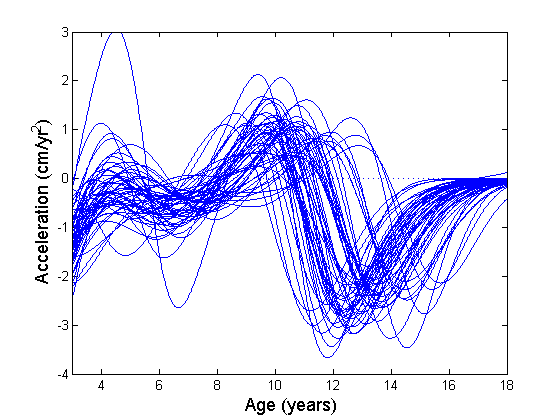
\includegraphics[width=4in]{figs/FemaleAccel.png}
\end{center}

\end{frame}

%  --------------------------------------------------------------------

\begin{frame}

\begin{center}
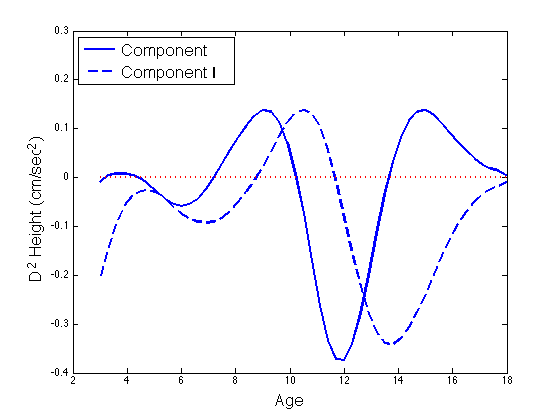
\includegraphics[width=4in]{figs/GrowthComponent_0.png}
\end{center}

\end{frame}

%  --------------------------------------------------------------------

\begin{frame}

\begin{center}
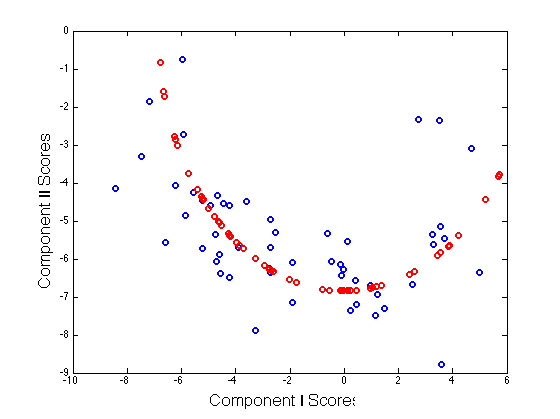
\includegraphics[width=4in]{figs/GrowthScore_0.png}
\end{center}

\end{frame}

%  --------------------------------------------------------------------

\begin{frame}

\frametitle{Regularized PCA of the children's acceleration curves}

\bi
  \item The principal component scores in $\Fbold$ are close to being on a circle,
  indicated by the red dots.
  \item We would like to explore the use of scores that are required to be close to or on the circle.
  \item The penalty term $\lambda_2 \| \Fbold  \Pbold_2 \Fbold' \|^2$, where projection matrix $\Pbold$ projects scores on to the circle of red dots, will serve that purpose.
  \item Here are the scores resulting from using $\lambda_2 = 1$.
\ei

\end{frame}

%  --------------------------------------------------------------------

\begin{frame}

\begin{center}
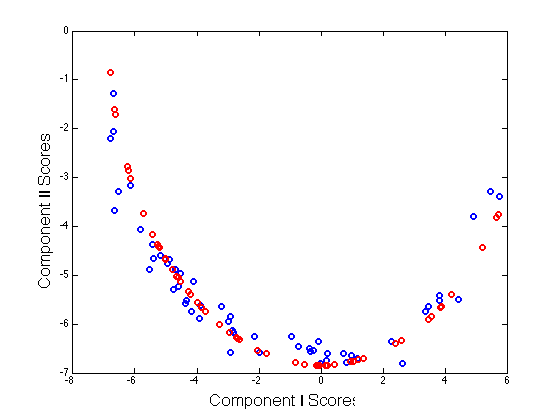
\includegraphics[width=4in]{figs/GrowthScore_1.png}
\end{center}

\end{frame}

%  --------------------------------------------------------------------

\begin{frame}

\bi
  \item The unconstrained error sum of squares was 127.2 and the contrained value was 138.2,
  corresponding to a squared multiple correlation of 0.08.  
  \item A heavier penalty puts the scores nearly exactly on the circle, corresponding to $R^2 = 0.12.$
  \item The angle associated with each pair of scores measures phase variation, which is how early or late the pubertal growth spurt is.
  \item But, we might have missed something ...
\ei

\end{frame}

%  --------------------------------------------------------------------

\begin{frame}

\begin{center}
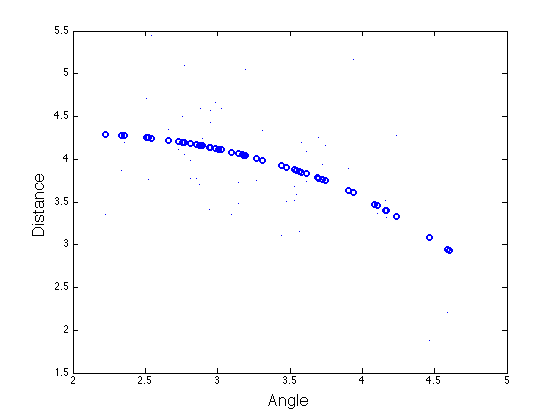
\includegraphics[width=4in]{figs/GrowthFSmooth.png}
\end{center}

\end{frame}

%  --------------------------------------------------------------------

\begin{frame}

\bi
  \item The scores of the girls in the upper left are outside of the constant distance curve, 
  and the girls on the bottom and lower right are inside.  
  \item The upper left girls have earlier puberty, and also more intense spurts;  the late puberty girls have milder growth spurts.  
  \item Early puberty girls are compensated for losing out on a few years of growth by having more intense spurts.
  \item It looks like principal component scores for uncentered functional observations should be represented in hyperspherical coordinates!
\ei

\end{frame}

%  --------------------------------------------------------------------

\begin{frame}

\frametitle{Conclusions}

\bi
  \item PCA via eigenanalysis restricts the extendability and versatility of PCA.
  \item Parameter cascading re-defines PCA as a much lower dimensional fitting problem,
  \item and greatly extends its capacity of represent data in a lower dimensional space.
\ei

\end{frame}

\end{document}
